\subsection{Switch String}

O suporte de \texttt{String} em \texttt{Switch} foi permitido em Java 7 este recuso ajuda a preservar um padrão de codificação tendo em vista que atualmente é permitido operações de seleção em um conjunto de constantes de \texttt{String}. Além de possuir desempenho superior ao \texttt{if-then-eslse} conforme a documentação~\cite{docSwitch} informa pois o gerado para \texttt{switch} que utilizam \texttt{string} é mais eficiente que o \texttt{if-then-else}.

Como contribuição deste trabalho foi feita uma pesquisa para verificar se tal recurso é adotado tendo em vista os benefícios que pode trazer para o projeto além de ser uma característica de fácil implementação. De um total de \num{6827} utilizações de \texttt{switch} nos sistemas apenas \num{66} fazem uso de \texttt{string} o que corresponde a menos de \num{1}\% do total o que leva entender que tal característica não é aproveitada em sua plenitude. A Tabela:~\ref{tab:adocaoSwitchString} exibe os projetos em houve ocorrência.


\begin{table}[ht] \footnotesize
	\centering
	\caption{Adoção \texttt{Switch String} por tipo do sistema.}
	\begin{tabular}{cc}
		\hline
		Sistema & Ocorrências \\ 
		\hline \hline
		\texttt{Cassandra} & 14 \\ 
		\texttt{FindBugs} & 3 \\ 
		\texttt{Jetty} & 16 \\
		\texttt{Lucene} & 2 \\
		\texttt{Sonar} & 1 \\
		\texttt{Spring} & 2 \\
		\texttt{Tomcat} & 8 \\
		\texttt{UniversalMediaServer} & 18 \\
		\texttt{Wicket} & 1 \\
		\texttt{Wildfly} & 1 \\	 \hline
		\texttt{Total} & 66 \\ \hline
	\end{tabular}
	\label{tab:adocaoSwitchString} %std means summary of type declarations
\end{table}


Com intuito de encontrar oportunidades de aplicar este recurso, foi verificado a existência de \texttt{if-then-else} que invoquem na sua expressão um método e verificando se este método utiliza o \texttt{equals("")} comparando \texttt{String} conforme demonstrado na Listing:~\ref{lst:demoIfEquals} o qual é a oportunidade possível de efetuar um  \textit{refectoring} para o \texttt{switch}.

\begin{lstlisting}[caption={Modelo para aplicação de \texttt{Switch} com \texttt{String}.}\label{lst:demoIfEquals},language=Java] 
if (String.equals("...")) {
...
}
\end{lstlisting}

Direcionado pelo padrão da Listagem:~\ref{lst:demoIfEquals} foram encontrados o total de \num{4940} oportunidades destribuidas em \num{45} dos \num{46} projetos, o que confirma que este recurso não está sendo adotado em sua plenitude. A Figura:~\ref{fig:oportunidadesSwitchString} exibe a quantidade de oportunidades em cada projeto verificado, e a Tabela:~\ref{tab:oportunidadesSwitchPorNatureza}.

\begin{figure}[h]
	\center
	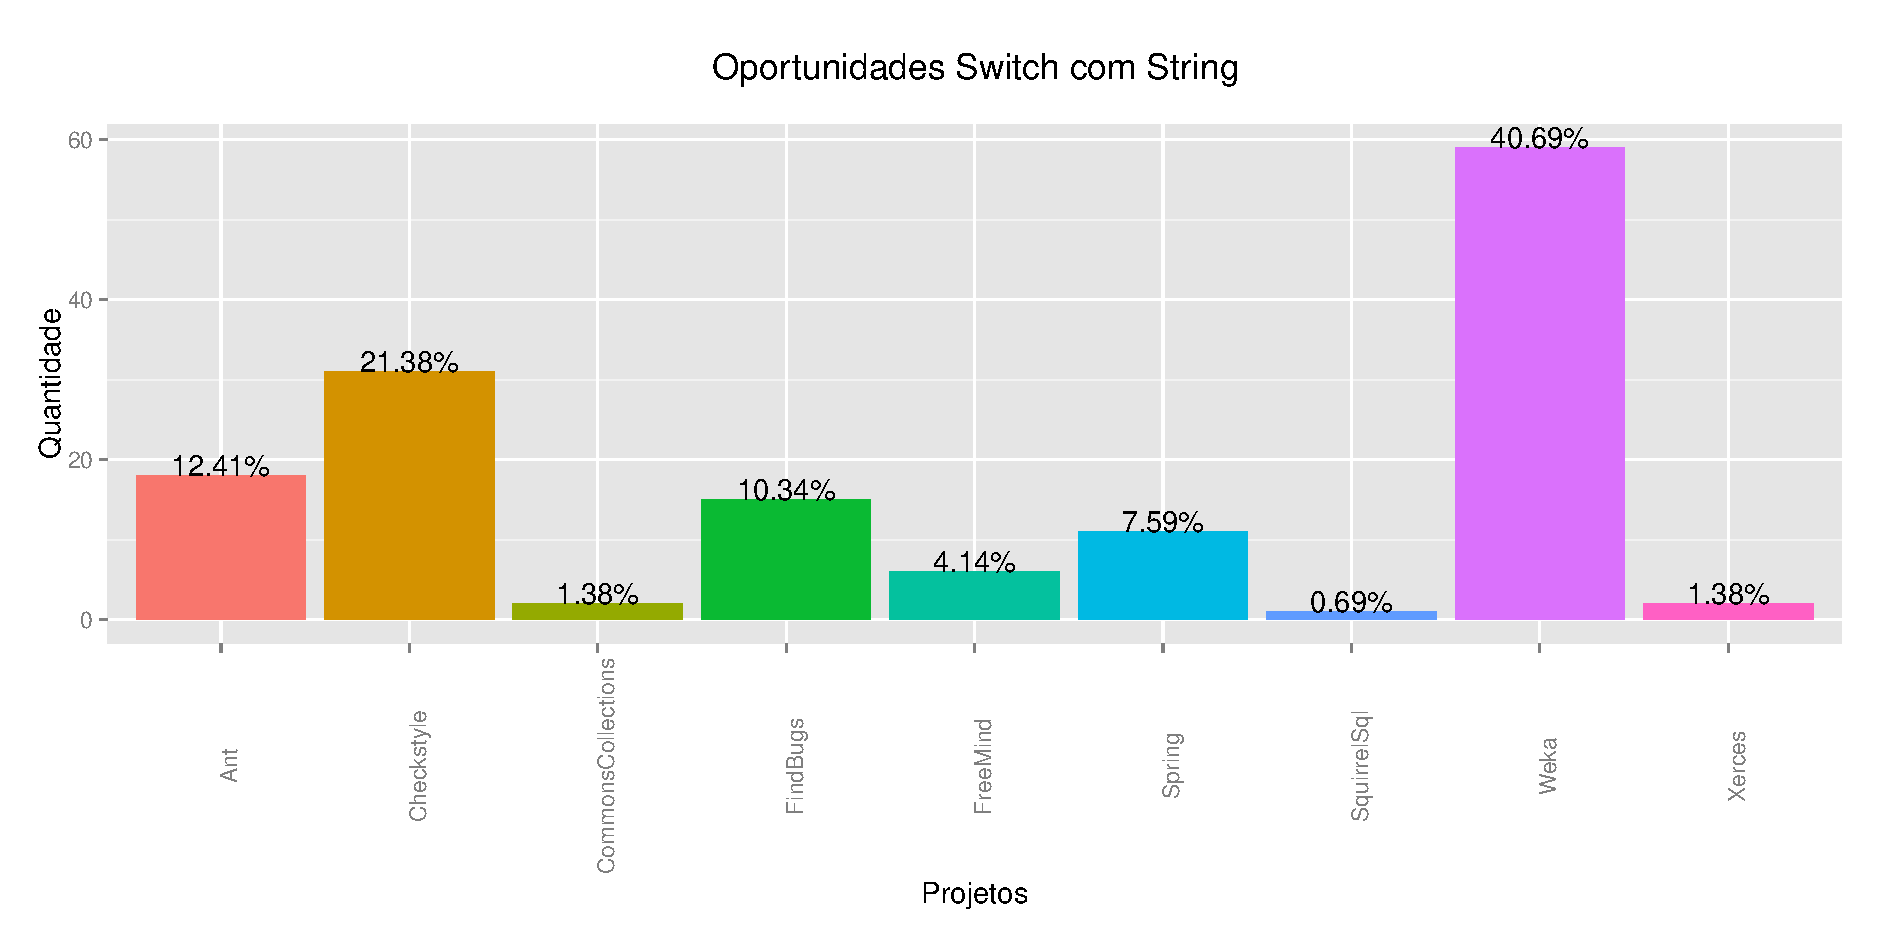
\includegraphics[scale=0.55]{Imagens/oportunidadesSwitchString}
	\label{fig:oportunidadesSwitchString}
	\caption{Oportunidades de \textit{refactoring} em \texttt{if-then-else} por sistema.}
\end{figure}


\begin{table}[h]
	\centering
	\caption{Oportunidade de aplicar \texttt{switch} por tipo de sistema.}
	\begin{tabular}{cc}
		\hline
		Natureza & Ocorrências \\ 
		\hline \hline
		\texttt{Application} & 1773 \\ 
		\texttt{Library} & 1881 \\ 
		\texttt{Servers - Database} & 1286 \\ \hline
		\texttt{Total} & 4940 \\ \hline
	\end{tabular}
	\label{tab:oportunidadesSwitchPorNatureza} %std means summary of type declarations
\end{table}



